\chapter{Evaluation of Visualization Methods}
\label{Chapter4}

In this chapter, we use the prototype implemented in chapter \ref{Chapter3} to conduct an experiment to evaluate the five visualization methods proposed in section \ref{VisualizationMethods}.

%------------------------------------------------------------------------------

\section{Evaluation Condition}

The experiment only focuses on the understandability evaluation. Other things like realtimeness, accuracy, and robustness as described in section \ref{VisualizationRequirements} are not considered.

Students of about 20--30 years old are invited to use the system with the five visualization methods. After that, each user is asked to rank the understandability of each visualization method in five levels of ranking points (1: worst, 5: best). Each user is forced to give unique ranking points across all five methods.

We have conducted the experiment outside the building of the College of Engineering Systems, at the area as in figure \ref{fig:VolumeMethod} and \ref{fig:SceneModel}:

\begin{itemize}
	\item Use the ``two keyframes'' method in section \ref{MapInitializing} to initialize the PTAM map.
	\item Each user points the mobile camera at the wall and see the visualized viewing field of one virtual camera. The user can change the position and/or orientation of the mobile. They can also walk around the area.
	\item The iPhone is used. The video frame size is 304 x 400, and is enlarged to 320 x 421 to fit the width of the screen. It operates at about 7 frame-per-second.
\end{itemize}

Figure \ref{fig:ExperimentScreenshot} shows a screenshot of the arrow visualization method. The users can use button 1--5 to switch among visualization methods, and button M to toggle between real and map viewing mode. The A button is for administration task, not used by the users.

\begin{figure}[htbp]
	\centering
	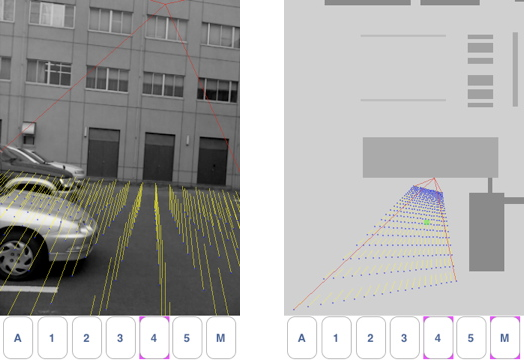
\includegraphics[width=14cm]{./Primitives/experiment_screenshot.png}
	\rule{35em}{0.5pt}
	\caption[Evaluation experiment screenshot]{Evaluation experiment screenshot of the arrow visualization method in real viewing mode (left) and map viewing mode (right)}
	\label{fig:ExperimentScreenshot}
\end{figure}

%------------------------------------------------------------------------------

\section{Result and Discussion}

The result is shown in table \ref{tb:ExperimentResult}. The numbers inside parentheses are points given by the users. The outside numbers are the average of the inside numbers.

\begin{table}[tb]
	\begin{center}
		\caption{Result of the evaluation experiment of visualization methods}
		\label{tb:ExperimentResult}
		\begin{tabular}{|c|c|c|c|c|}
			\hline
			Method    & Understandability \\
			\hline
			Volume    & 1.0 (1 1 1 1 1) \\
			Shadow    & 3.2 (3 4 2 4 3) \\
			Contour   & 2.2 (2 2 3 2 2) \\
			Arrow     & 4.2 (5 3 4 5 4) \\
			Animation & 4.4 (4 5 5 3 5) \\
			\hline
		\end{tabular}
	\end{center}
\end{table}

The most preferred visualization methods are the arrow and animation method. A good visualization method is the one in which the visual aids do not occlude the scene. The arrows and the moving mesh are constantly displayed on the screen but do not occlude the scene over time, hence they give the best understandability. Moreover, this method also points out where the surveillance camera. On the contrary, the visual aids by the volume method is the worst because its CG object usually occludes large parts of the screen.

We have only conducted the experiment in a small outdoor area with the viewing field of one surveillance camera. More extensive experiments in various conditions, such as larger areas, more surveillance cameras, overlapping viewing fields etc. should be conducted before more solid conclusion could be made. In those conditions, methods with non-animated visual aids may be of less understandability because the visual aids may have similar color with the color of the texture of the real scene, or they overlap with one another.

The understandability is largely affected by the way we draw the visual aids. In previous experiments, we did not draw the four straight lines as described at the begin of section \ref{VisualizationMethods}, and the users could hardly understand the shadow and contour methods. Colors of the visual aids may also affect the understandability. Currently the visual aids are drawn semi-transparent:

\begin{itemize}
	\item Blending function: result color = 0.5 x source color + 0.5 x destination color
	\item The four boundary lines of the viewing field are drawn in red
	\item The visual aids at the sides or inside the viewing field are drawn in yellow, and green
	\item The buildings are drawn in gray
\end{itemize}

These colors are bright hot and have good contrast, hence users can easily differentiate the different elements. In previous experiments, we used dark colors and users had bad feelings about the visual aids.

A good gene is usually a mixture of pure gene or other mixed gene. Likewise a good visualization can be a combination of various methods. In the future we should try to combine the methods to find ones better than the current methods.
